% \documentclass{llncs}
% \documentclass[USenglish,onecolumn,11pt]{article}
\documentclass[conference]{IEEEtran}
\usepackage[margin=1in]{geometry}
\usepackage{amsmath,algorithm}
\usepackage[dvipsnames]{xcolor}
\usepackage{algpseudocode}
\usepackage{graphicx}
\usepackage{amsmath}%
\newtheorem{theorem}{Theorem}
\newtheorem{axiom}[theorem]{Axiom}
\newtheorem{lemma}[theorem]{Lemma}
\newtheorem{claim}[theorem]{Claim}
\newtheorem{remark}{Remark}
\newtheorem{exercise}{Exercise}
\newtheorem{definition}{Definition}
\newtheorem{example}{Example}
\newcommand{\PAccess}[1]{\mathsf{Access}_\Sigma(#1)}
\newcommand{\ORequest}[1]{\stackrel{\rightarrow}{#1}}
\newcommand{\newText}[1]{{\color{Red}#1}}
\newcommand{\norm}[1]{\lvert#1\rvert}
\newenvironment{todo-text}{\color{Red}}{\hfill}
\newenvironment{newtext}{\color{ForestGreen}}{\hfill}
\newenvironment{proof}{\paragraph{Proof:}}{\hfill}
\begin{document}
\title{Using SGX for Bitcoin Simplified Verification Payment Client}
\date{}
\maketitle              % typeset the title of the contribution
\begin{abstract}
% \keywords{Intel SGX, Path ORAM, Bitcoin}
\end{abstract}
%
%!TEX root = main.tex
\section{Introduction}
\label{sec:introduction}
Over the last few years, we have seen a great interest in public blockchain in the community. 
Bitcoin blockchain technology offered a way to provide security and privacy for financial transactions. 
However, with a huge adoption by the community, the size of the blockchain has become too large for small and resource-constrained devices such as personal laptops or mobile devices.
\begin{newtext}
As of June 2018, the size of unindexed Bitcoin blockchain is 180 GB.
\end{newtext} 

Bitcoin simplified payment verification (SPV) client has become one of the solutions for storage problem for constrained devices. 
Nakamoto~\cite{Nakamoto_bitcoin:a} sketched the idea of SPV clients in the Bitcoin whitepaper, 
and in the Bitcoin improvement proposal 37 (BIP37)~\cite{BIP37}, Mike Hearn combines Nakamoto's idea with Bloom filter to standardize the design of Bitcoin SPV clients. 
This design has become de facto standard and used by other light clients such as BitcoinJ and Electrum.

SPV clients only need to download and verify part of blockchain that is relevant to its addresses. 
In particular, the SPV client loads its addresses into a Bloom filter and sends the filter to a bitcoin full client. 
The Bitcoin full client will use that filter to identify if a block contains transactions that are relevant to the SPV client, 
and once it finds such block, it will send a modified block that only contains relevant transactions along with Merkle proofs for those transactions. 
\\
\textbf{Limitation. }
Gervais et. al.~\cite{Gervais:2014:SPV-privacy} show that it's possible for a malicious node to learn several addresses loaded in the Bloom filter with high probability.
If the adversial node can collect 2 filters issued by a same client, then a considerable number of addresses owned by that client will be leaked.
Moreover, full nodes that supports the use of Bloom filter are targeted for Denial-of-Service attacks as the malicious clients can cripple it by making lots requests that cause high CPU usage on the full clients \cite{spv-dos}.
\\
\textbf{Our Solution. }
We propose a design for a centralized system that can handle transaction requests from Bitcoin simplified payment clients while offering strong security and anonymity guarantees agaisnt potentally malicious providers. In particular, our design use standard ORAM scheme with a hardware-based solution to protect client's requests from a potentially malicious server.
\\
% \begin{todo-text}
% 	\begin{itemize}
% 		\item request distribution

% 		\item batch writing 

% 		\item untrusted Bitcoin client can delay incoming blocks which the update enclave stucks in updating process.
% 	\end{itemize}
% \end{todo-text}

%!TEX root = main.tex
\section{Related Work}
\label{sec:related-work}
\begin{todo-text}
(write this)
\end{todo-text}
%!TEX root = main.tex
\section{Preliminaries} % (fold)
\label{sec:preliminaries}

\subsection{Oblivious Random Access Memory} % (fold)
\label{sub:oblivious_ram}
Oblivious Random Access Memory (ORAM) concept was first introduced by Goldreich et al~\cite{Goldreich:1987} for software protection against piracy. The main idea of ORAM is to hide the access patterns resulted by reading and writing accesses on encrypted data. The security of ORAM can be described as
\begin{definition}~\cite{Stefanov:2013}
	Let
	$\stackrel{\rightarrow}{y}=(\mathsf{op_i,a_i,data_i})_{i\in [n]}$
	denote a sequence of accesses 
	where $\mathsf{op_i}\in \mathsf{\{read,write\}}$, 
	$\mathsf{a_i}$ is the identifier, 
	and $\mathsf{data_i}$ denotes the data being written. 
	For an ORAM scheme $\Sigma$, let $\mathsf{Access}_{\Sigma}(\stackrel{\rightarrow}{y})$ denote a sequence of physical accesses pattern on encrypted data produced by $\stackrel{\rightarrow}{y}$.
	We say:
	\begin{enumerate}
	  	\item The scheme $\Sigma$ is secure if for any two sequences of accesses $\stackrel{\rightarrow}{x}$ and $\stackrel{\rightarrow}{y}$ of the same length, $\PAccess{\ORequest{x}}$ and $\PAccess{\ORequest{y}}$ are computationally indistinguishable.
	  	\item The scheme $\Sigma$ is correct if it returns on input $\ORequest{y}$ data that is consistent with $\ORequest{y}$ with probability $\geq 1 - \mathsf{negl}(\lvert\ORequest{y}\rvert)$
  	\end{enumerate}
\end{definition}
\textbf{Path-ORAM.}
Path-ORAM is an efficient tree-based ORAM construction proposed by Stefanov et. al. \cite{Stefanov:2013}. 
In Path ORAM, the client encrypts his database into $N$ different encrypted data blocks, 
and uses a binary tree of height $L$ to obliviously store those data blocks into a server's untrusted storage. 
Each node of the tree is a \textit{bucket} that can store at most $Z$ blocks. 
The client uses a \textit{position map} to keep track of the location for each real data block. 
For any read and write accesses performed on the encrypted database, the client requires to perform a read, an eviction, and an update procedure on the tree and on the position map. 
In particular, in order to perform an access on a block, the client uses the position map to look up the block's position in the binary tree to obtain its path, and the client retrieves the path from the server, decrypts, and stores the whole path in a local \textit{stash} of size $O(\lambda)$ blocks where the parameter $\lambda$ denotes the security level which defines the overflow probability and security level of the path ORAM. 
The client looks up the targeted block in the stash, and perform access on it. 
Finally, the client assigns the target block with a new random path, and push all blocks in stash back to the tree according to the position map. 
Figure~\ref{fig:oram-access} describes in detail a Path-ORAM access. 

Using same notations in~\cite{Stefanov:2013}, we denote $\mathcal P(x)$ to be the path from the leaf $x$ to the root. $\mathcal P(x,\ell)$ denote the bucket at level $\ell$ along the path $\mathcal P(x)$. $\mathsf{ReadBucket(b)}$ denotes decrypting and reading all blocks from bucket $b$. Similarly, $\mathsf{WriteBucket}(b,\mathsf{Block}')$ denotes encrypting and writing block $\mathsf{Block}'$ into bucket $b$. $\mathsf{Position}[\cdot]$ denotes the position map, and $\mathsf{Position[a]}$ outputs the path identifier that block with $a$ is stored. Finally, $S$ is the stash that is stored on client side.
\\
{
\begin{figure}[!h]\label{fig:oram-access}
	\centering
	\begin{minipage}{\linewidth}
	\begin{algorithm}[H]
	  	\caption{$\mathsf{Path\text{-}ORAM.Access(op,a,data^*})$\label{alg}}
	  	\begin{algorithmic}[1]
			\State $x \leftarrow \mathsf{Position}[a]$
			\item $\mathsf{Position}[a] \stackrel{\$}{\leftarrow} \{0,\dots,2^L-1\}$ 
			\For{$i \in \{0,\dots, L\}$}
			\State {$S \leftarrow S \cup \mathsf{ReadBucket}(\mathcal P(x,\ell))$}
			\EndFor
			\State $\mathsf{data}\leftarrow$ read block $a$ from $S$
			\If{$\mathsf{op = write}$}
			\State $S \leftarrow (S - \mathsf{\{(a,data)\}\cup \{(a,data^*)\}})$
			\EndIf
			\For{$\ell \in \{0,\dots, L\}$}
			\State $S'$ $\leftarrow$ $\{$ $\mathsf{(a',data')}$$\in$$ S$$:\mathcal{P}(x,\ell)=\mathcal{P}(\mathsf{position[a'],\ell})$$\}$
			\State $S' \leftarrow$ Select $\min(S',Z)$ blocks from $S'$
 			\State $S \leftarrow S - S'$
			\State $\mathsf{WriteBucket}(\mathcal{P}(x,\ell,S'))$
			\EndFor
			\State \Return $\mathsf{data}$
		\end{algorithmic}	
	\end{algorithm}
	\end{minipage}
	\caption{a Path-ORAM access}
\end{figure}
}
\textbf{Recursive ORAM.} 
In the non-recursive Path-ORAM construction, the client has to store a position map of the size $O(N)$ bits. 
This is not suitable for a resource-constrained client. Stefanov et. al~\cite{Stefanov:2013} and Shi et. al.~\cite{Elaine-rORAM} present path ORAM construction that reduces the size of the position map to $O(1)$. 
The main idea of those constructions is to store a position map as another ORAM tree in the server side, and the client only keeps the position map of the new ORAM.
The client keeps compressing the position map into another ORAM tree until the size of position map is small enough to be kept client's storage. 
These constructions come with the cost of an increase in communication between client and server. 
% However, for this work, if we consider the Intel SGX to be the client in ORAM setting, then the cost of communication is the IO access between SGX and the random access memory. 
In this work, we consider the Intel SGX as the client in the ORAM protocol; therefore, the total size of the position map and stash is limited by the size of EPC which is around $128$MB. Thus, recursive path ORAM might be a suitable solution for a large dataset. 

\subsection{Intel SGX} % (fold)
\label{sub:intel_sgx}
Intel SGX is a set of hardware instructions introduced with the 6th Generation Intel Core processors. 
We use Intel SGX as a trusted execution environment for the execution of ORAM controller on the untrusted server. 

In this project,  we focus on these main properties of Intel SGX:
\noindent 
\begin{itemize}
	\item \textbf{Enclave:} is the trusted execution unit that is located in a dedicated portion of the physical RAM. The Intel SGX makes sure that all other software on the system cannot access the enclave memory. 
	\item \textbf{Remote Attestation and Key Exchange:} 
	SGX allows a remote client to perform a remote attestation to verify the correct creation of an enclave. 
	More importantly, the remote attestation provides an authentication needed for an authenticated key exchange protocol \cite{sgx-explained}. 
	In particular, after a remote attestation,  a client can use Diffie-Hellman Key Exchange~\cite{DH-keyexchange} to agree on a shared secret.

	\item \textbf{Local Attestation: } Local attestation allows two enclaves on the same system to authenticate each other and exchange data in a secure manner.
\end{itemize}
\textbf{Limitations.}
There are several weaknesses of the Intel SGX
\begin{itemize}
	\item \textbf{Side Channel Attacks:} While Intel SGX provides security guarantees against direct memory attacks, it suffers from various side-channel attacks \cite{Xu15ControlledChannel,asyncshock,BrasserMDKCS17,hid-sgx-sidechannel-usenix17,shadow-branch-lee-usenix17}. 

	\item \textbf{Enclave Page Cache Limit:} The size of EPC is limited to around $128$MB~\cite{Arnautov-epc}. 
\end{itemize}

\begin{todo-text}
\paragraph{Secure Oblivious Operations} % (fold)
\label{par:secure_operations}
	discussion on oblivious comparision, oblivious assignment here. 
	oevict,  oreadpath in zerotrace.
\end{todo-text}
% paragraph secure_operations (end)

\subsection{Bitcoin Unspent Transction Output Database}
Each Bitcoin transaction contains inputs and outputs. 
Thus, a Bitcoin client can determine its balance by summing up all values in those outputs that have not been spent.
These outputs are called Unspent Transaction Output (UTXO).
% Instead of scanning the whole blockchain to verify transactions, 
Moreover, Bitcoin full nodes maintain a separate database that keeps track of all unspent transaction outputs. 
This approach allows a full client to fast validate unconfirmed transactions before relaying it to other nodes. 
More importantly, the UTXO set stores all information needed for client with knowledge of a secret key to create a new transaction. 
Therefore, we realize that:
\begin{itemize}
	\item \textbf{Privacy}: If the server can provide the SPV client oblivious accesses to the UTXO set, the privacy of the SPV client is preserved.
	% \item \textbf{Scalability}: If there is a way to authenticate the client before providing accesses to the UTXO set, the system will be safe from some trivial DDOS attack. 
	% By providing limited accesses on the unspent transaction output, we  
\end{itemize}
% subsection intel_sgx (end)
% subsection oblivious_ram (end)
% section preliminaries (end)
%!TEX root = main.tex
% \section{Design}

\section{Proposed System} % (fold)
\label{sec:new-protocol}
In this section, we describe how to use Intel SGX as trusted execution unit and Path ORAM to allow a remote client to access the UTXO set in an oblivious manner.

\subsection{Overview} % (fold)
\label{sub:overview}
There are 3 components of this system: a client, a untrusted server, and the Bitcoin network. In the untrusted server, we require that there exist two secure enclaves: one for read and one for update.
\begin{itemize}
	\item \textbf{Client} is the simplified payment verification node that remotely connects to the secure enclave on the untrusted server to perform oblivious searches on the UTXO set.

	\item \textbf{Server} is the untrusted entity that is made up of three components: an untrusted OS, a secure trusted read enclave, and a secure trusted update enclave. In particular, the secure update enclave communicate to the Bitcoin network in order to initialize and update the ORAM tree. Moreover, SPV clients can connect to the read secure enclave to invoke ORAM read operations on the ORAM tree to obtain its unspent output.

	\item \textbf{Bitcoin Network} is a set of nodes that maintain the Bitcoin blockchain and relays the new Bitcoin block validated by miners.
\end{itemize}
The system will works as follow:
\begin{itemize}
 	\item \textbf{Initialization:}
	Since there is no protection from the SGX on system calls such as Network I/O, 
	we expect that the Bitcoin client that runs in the untrusted OS will perform the communication with the Bitcoin network to obtain the Bitcoin blockchain data.
	Fortunately, Bitcoin uses proof-of-work for its consensus protocol, 
	so we argue that the Bitcoin client reside untrusted OS cannot fool the enclave into using different blockchain because it will have to perform enormous amount of computation power to reproduce a blockchain of same length. 
	First, the enclave will first initialize an empty ORAM tree. 
	Then, for each of Bitcoin block, the enclave will verify the proof of work of the block before using ORAM update operations to populate the ORAM tree. 
	This operation might take several hours. 
	However, once the SGX catches up with the current state of the Bitcoin blockchain, we expect that the enclave only has to perform a batch of update accesses on the ORAM tree every 10 minute.

	\item \textbf{Search Query:} In order to obtain its unspent outputs, the client first performs the remote attestation to the enclave. 
	As mentioned in the previous section, the remote attestation process allows the client to verify if the program is correctly loaded into the enclave or not. 
	More importantly, during the remote attestation, the client can share a secret session key with the enclave to establish a secure connection using \textit{mbed-tls} in SGX. 
	Next, after establishing a secure channel, the client will send a list of hash preimages to the enclave. 
	The read enclave will use a mapping function that map those the preimages to the ORAM block identification and perform ORAM read-only operations on the ORAM tree. 
	In particular, those read-only operations do not involve the eviction procedure which requires reencrypting and remapping ORAM block. 
	We will describe the intuition and the security of this operation in section \ref{sub:oRAM operations}.
	% Intuitively, we don't want read operations to be blocked by ongoing update operations. There will be a read copy of the ORAM tree that is dedicated to handle requests from the client and a shadow copy of ORAM tree where all real ORAM operations will be performed on.

	\item \textbf{Update Query:} 
	It has been reported that the throughput of Bitcoin network is 3-7 transactions per second \cite{scaling-blockchain-3-7}. 
	Every input of a transaction implies a deletion operation or an ORAM update operation with dummy data, 
	and every new output means another update operation on the ORAM tree. 
	We estimate that there are an 14 inputs and outputs on average in a Bitcoin transaction (as of January 2018). 
	Thus,  an ORAM implementation using Intel SGX can easily handle 14 ORAM operations per second.
	% Thus, with the  the Intel SGX can obviously support 14 ORAM operations per second. 
	However, due to the Bitcoin proof-of-work consensus protocol, the Bitcoin network generates a new block approximately 10 minutes. 
	The system will expect a batch of update operations every 10 minutes instead of every 14 operations every seconds. 
	Therefore, in order to prevent updating operations from being blocked by read requests from client, 
	we require that there must be two copies of the ORAM trees: a read-only tree and a shadow-copy tree, 
	and there is an dedicated update enclave that performs a batch  of write accesses every 10 minute.
	Then, when a batch updating operations are finished, we update the position map and the read-only tree with the shadow-copy tree.
	% While there are several solution for concurrency problems for ORAM \cite{taostore,curious}, we 

\end{itemize} 
% subsection overview (end)

\subsection{Oblivious Storage of the UTXO set}
\label{subsec: Oblivious Storage of the UTXO set}
In this work, we only consider 2 types of transaction: \texttt{Pay-to-Pubkey-Hash} transaction and $\texttt{Pay-to-Script-Hash}$ transaction.
According to \cite{analysis-of-utxo}, these two types of transaction make up of $99.1\%$ of the UTXO set. 
Also, one can assume that the \texttt{Pay-to-Pubkey-Hash} transaction is a special version of the \texttt{Pay-to-Script-Hash} transaction 
because both transaction types require the spender to know the preimage of the hash digest before being able to spend those outputs.  
Each of those output contains a hash digest of length 160 bit.
% Also, those unspent outputs that belong to those transactions can be uniquely identified by the $160$-bit hash digest.
% As of April 2018,  the number of unspent outputs belong to \texttt{Pay-to-Pubkey-Hash} is around $44,000,000$ outputs. We found out that these outputs make up $84\%$ of all UTXOs.
% Each UTXO takes about $68$ bytes. 

In this system, those outputs belong to \texttt{Pay-to-Pubkey-Hash} and \texttt{Pay-to-Script-Hash} will be partitioned into different data blocks and stored as a tree structure in the memory of the untrusted server. 
Thus, there must be a way to map the hash digest in each output into ORAM block identification.

If we consider each unspent output as one ORAM block in the ORAM tree and use the hash digest as the ORAM block identification, the position map will become too big for the EPC memory because the size of each identification key is 20 bytes.
Another way is to use a standard hash function that provides a mapping between public key hash and ORAM block identification (e.g. $H:\{0,1\}^{160} \rightarrow \{0,1\}^{32}$). However, directly hashing public key hash into ORAM block identification is not suitable because an attacker can generate several public keys which the hash digests map to the same ORAM block, then fills those public key with small amount of bitcoin. 
The block will become overflow, and those unspent outputs of legitimate users will be discarded.

To avoid such attack, in our design, during the initialization, we require the program inside the enclave to use a keyed hash function to map the public key hash to ORAM block identification. The secret key of the hash function is stored inside the enclave.  
In other word, the mapping between the public key hash and the ORAM block identification is known only to the SGX. 
We define the mapping as follow:
\begin{itemize}
	\item $\mathsf{bid}\leftarrow blockMapping(\mathsf{hd}, K_b)$: It takes as input a hash digest $\mathsf{hd}$ and a secret key $K_b$, it outputs the block identification number $\mathsf{bid}\in \{0,\dots,N-1\}$. The value $m$ will determine the maximum number of unspent outputs packed in one block and the size of the position map. We will analyze and show how to choose an appropriate value of $m$ later. 
\end{itemize}
This approach, however, does not entirely prevent an attacker from populating a single address with lots of unspent outputs which also causes an ORAM block to overflow.
Fortunately, after analyzing the UTXO set, we find out that around $95\%$ of all bitcoin addresses owned less than 5 unspent outputs. 
Thus, if we limit the number of unspent outputs for each public key to $5$, we can accommodate $95\%$ of all bitcoin users and avoid the above attack. 
Figure \ref{fig:utxo-analysis} shows us the distribution of unspent outputs and bitcoin address.
\begin{figure}[H]
	\centering
	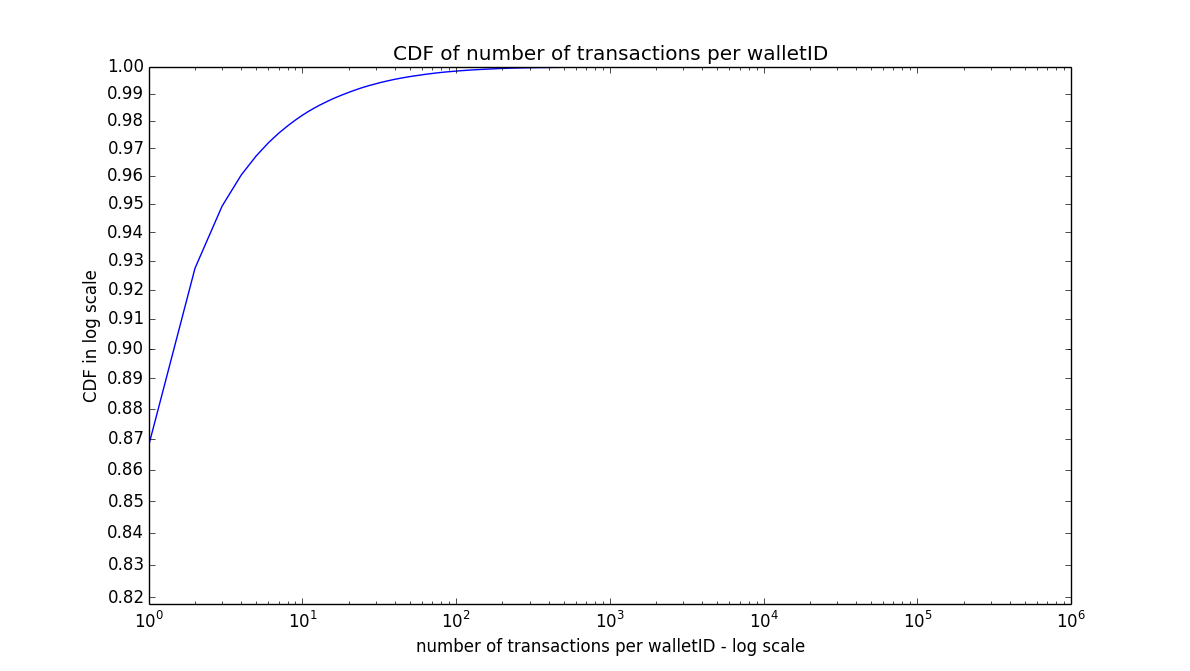
\includegraphics[width=\linewidth]{fig/cdf.png}
	\caption{Number of transactions per wallet id}
	\label{fig:utxo-analysis}
\end{figure}

The hashing approach gives us some flexibility between the size of an ORAM blocks and the size of the position map stored inside the enclave. However, it also comes with the cost of additional storage in the server. The following claim gives us a loose upper bound of the number of addresses can be stored inside an ORAM block.
\begin{claim}(Addresses per ORAM block)\label{claim:addressesperoramblock}
	Let $m$ be the number of public keys,  $N$ be the number of ORAM blocks. If the $blockMapping(\cdot,\cdot)$ acts a truly random function, then the maximum load of each ORAM block is smaller than $e\cdot m/N$ with probability at least $1 - 1/N$
\end{claim}
\begin{newtext}
\begin{proof}
	This is a standard bin and ball analysis.
	 % Let $X_1, \dots, X_m$ to be the random variable  that 
\end{proof}
\end{newtext}

\begin{newtext}
Thus, if we limit each ORAM block to contain the outputs of at most $e\cdot m/N$ addresses, then the probability that every address is included is at least $1-1/N$.
We let $\delta$ to be the number of unspent outputs each address can have and $\alpha$ be the size of each unspent output in bytes. The size of each ORAM block is  $e m  \delta \alpha/N$ bytes. 
Table \ref{tbl:delta} shows us the trade-off between the choice of $\delta$ and the required storage of $N$ ORAM blocks and the unspent output database coverage.
\end{newtext}
	% If we let each of $N$ ORAM block can contains at most $\ell$ addresses and each address to have at most $\delta$ unspent output of size $\alpha$ bytes, then we need to store $N\ell\delta\alpha$ bytes
	% If we allow each public key hash address to hold at most $\delta$ unspent output and each output require $\alpha$ bytes, then we need to store at least $\delta \cdot e \cdot m \cdot \alpha$ bytes
	% N blocks , each block holds $e\cdot m/N$ addresses, each address holds $\delta$ outputs. So in total we need: $N\cdot e\cdot m/N \cdot \delta \cdot 68 = \delta \cdot e \cdot m \cdot 68$ bytes
	% there are $N$ blocks, each block holds $e \cdot m/N$ address,  each addressso in total we needs: $$
\\
\begin{table}[!h]
\centering
\resizebox{\columnwidth}{!}{%
\begin{tabular}{c|c|c|c|c|c|}
	\hline
    \multicolumn{1}{|c|}{$\delta$}                                				& 1         & 2         & 3        & 4        & 5     \ \\ \hline
    \multicolumn{1}{|c|}{UTXO coverage}              			  				& $86\%$    & $91\%$    & $92\%$   & $94\%$   & $95\%$\ \\ \hline
    \multicolumn{1}{|c|}{Storage, $\alpha = 68$ bytes}           				& 3GB       & 6GB       & 9GB      & 12GB     & 15GB  \ \\ \hline
\end{tabular}
}%
\caption{Trade-off}
\label{tbl:delta}
\end{table}
\begin{newtext}
\begin{remark}
	The choice of $N$ does not affect the data size of the ORAM tree. 
	However, it determines the size of the ORAM block and the height of the tree.
	Thus, it decides the size of the position map for a non-recursive ORAM construction, 
	and the number of recursion levels for a recursive ORAM construction	
	We will show the experiment result for the optimal choice of $N$.
\end{remark}
\begin{remark}
	% variable-size oram by daniel roche
	% Our system currently uses path-ORAM and circuit-ORAM as the proof of concept t
	Notice that the system requires large extra storage in order to increase the upper limit of unspent outputs for each address. 
	The reason is because in most ORAM schemes, the size of ORAM block is fixed; therefore, we need to pad dummy data to each ORAM block. 
	However, Roche et. al.~\cite{roche-voram} proposed an ORAM scheme that allows to have different size block. 
	Their construction is a direct extension of non-recursive Path ORAM.
	Therefore, we believe that it is possible to overcome the storage requirement by using Roche's ORAM scheme.
	However, in this work, we only use path ORAM as the proof-of-concept for the design of our system.
\end{remark}
\end{newtext}

Finally, in this system, the untrusted server stores two ORAM trees: a read-only tree and a shadow-copy tree: 
\begin{itemize}
	\item \textbf{Read-only Tree} serves as a dedicated storage to handle client requests. While the structure of the tree is identical to the standard ORAM tree, the read-only access does not perform the eviction procedure on the tree like in a standard ORAM setting. 
	In other word, the read-only tree remains the same for the time interval of 10 minutes, and this approach limits the client to perform at most one read per public key every 10 minutes.
	\item \textbf{Shadow-copy Tree} is where all standard ORAM eviction operations are performed. 
	In particular, when the read enclave receives a request from the client, 
	it signals the update enclave to perform standard ORAM reads on the shadow-copy tree by sending a batch of ORAM block IDs via a secure channel; 
	this process can be done after a local attestation between two enclaves. 
	% When a new Bitcoin block arrives, the update enclave signals the read enclave to queue up all the read requests from the clients and performs all update requests.
	% Once the update operation is done, the update enclave signals the read enclave to update the new database and sends the new position map to the read enclave. 
	As a new Bitcoin block arrives, the update enclave perform all update operations on the shadow-copy tree, and once the update is finished, it signals the read enclave to use the shadow-copy tree as the new read-only tree. 
\end{itemize}
\subsection{UTXO Oblivious Read and Update Protocols}
\label{sub:oRAM operations}
In this protocol, the SPV client is the party who performs read accesses, and the Bitcoin network is the party who performs write accesses. 
The SGX in the server is the one that performs both of those accesses on behalf of the client and the Bitcoin network.

\subsubsection{Oblivious Read Protocol}
We will describe how a remote client can perform a read access on the UTXO set. 
We denote $K_s$ to be the session key, $K_o$ to be the ORAM key, $K_b$ to be the block mapping key, $R$ to be the response stash, $\mathsf{bid}$ to be ORAM block id and $PK_\mathsf{bid}$ be the set can be uniquely identified by the $\mathsf{bid}$. 
Figure \ref{fig:overview-read} gives an overview of this process.
\begin{figure}[t]
	\centering
	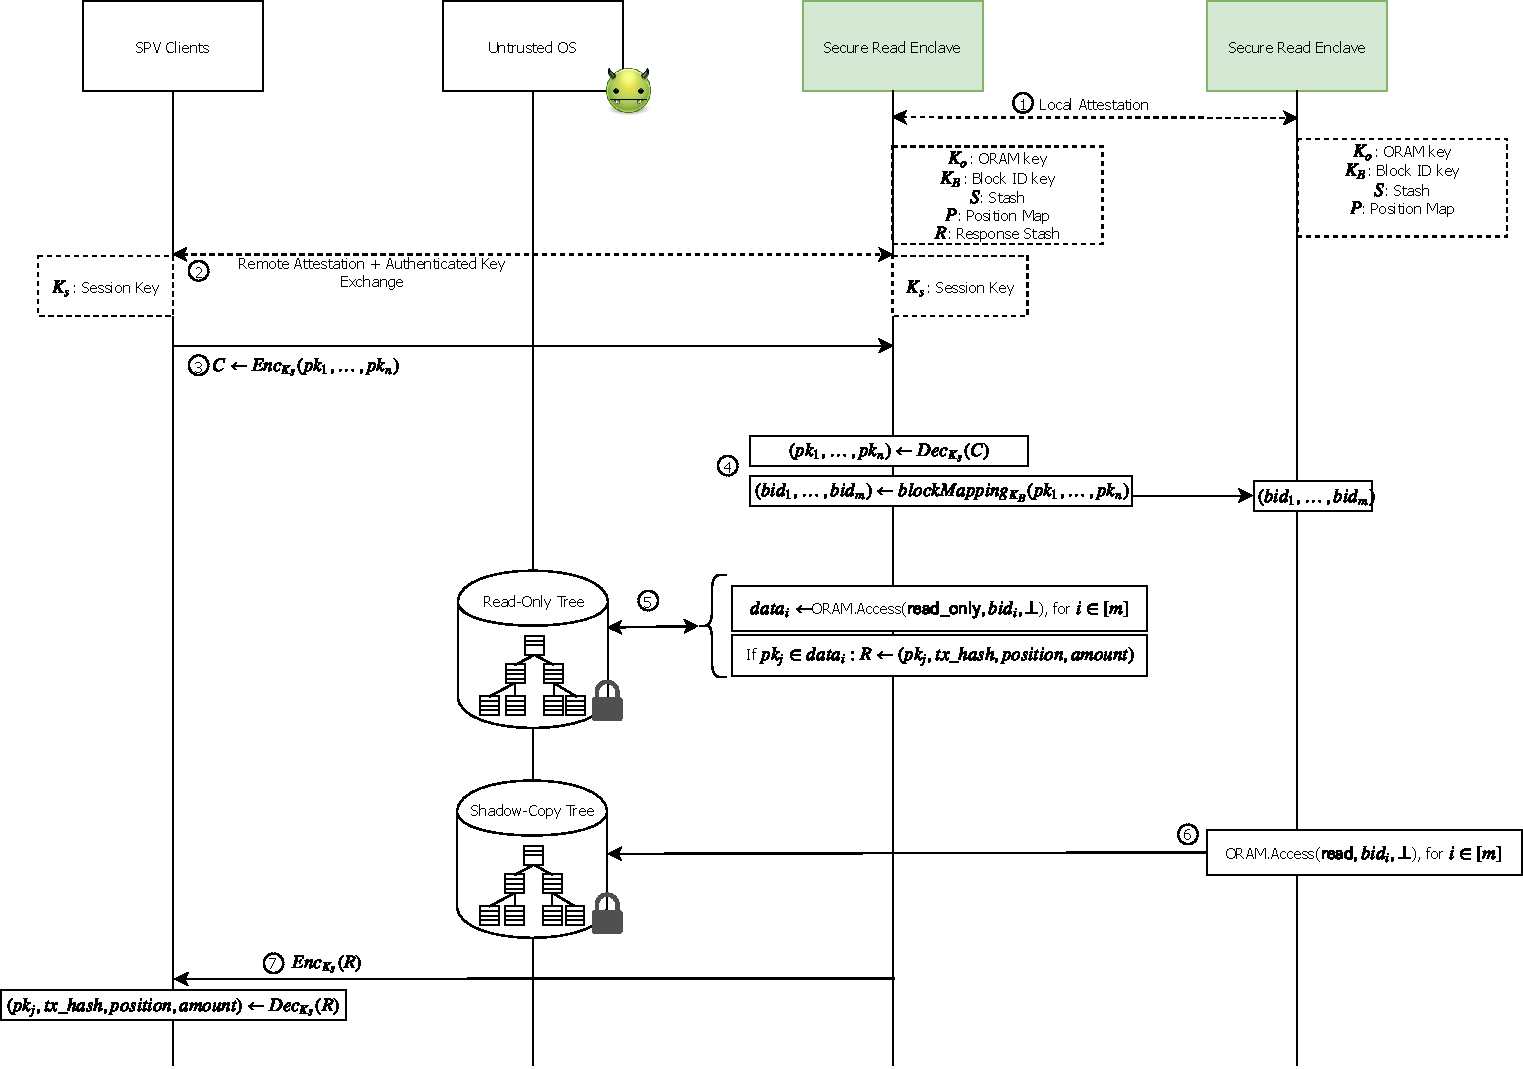
\includegraphics[width=\columnwidth]{fig/Client-Read.pdf}
	\caption{Oblivious Read Operation}
	\label{fig:overview-read}
\end{figure}
\begin{enumerate}
	\item \textbf{Establish Secure Channel: } First, the client performs a remote attestation with the secure read enclave and agrees on a session key, $K_s$.

	\item \textbf{Prepare Read Query:} The client encrypts its list of public keys or preimages of the hash digests and sends the encrypted query to the server to be passed to the enclave. For simplicity, we assume that the plaintext only contains a list of public keys that the client is interested in, $C$$\leftarrow$$Enc_{K_s}(pk_1,\dots, pk_n)$

	\item \textbf{Identify and Forward ORAM Block ID:} After decrypting the ciphertext $(pk_1, \dots, pk_n)$$\leftarrow$$Dec_{K_s}(C)$, the read enclave uses $blockMapping(\cdot,\cdot)$ function to learn which block may contain those public key, $(\mathsf{bid}_j)_{j\in[m]} \leftarrow blockMapping(pk_i, K_b)$ for each $i \in \{1,\dots, n\}$ where $K_b$ is the secret key stored in enclave for mapping purpose. After obtain a list of ORAM $(\mathsf{bid})_{j \in [m]}$, the read enclave forward  the list to the update enclave via a secure channel.

	\item \textbf{Perform ORAM read-only accesses on read-only tree:} Based on the given blockID and the public key, the enclave uses the $K_o$ to perform standard ORAM read accesses on the ORAM tree. If the block contains the unspent output that is related to the public key, we add it into  the response stash $R$. Figure \ref{fig:oram-read-only-access} describes the read-only operation. Also, we note that in this operation the read enclave only bring a copy of the path into the stash. This allows different enclave to handle different requests from different clients.

	\begin{figure}[t]\label{fig:oram-read-only-access}
	\centering
	\begin{minipage}{\linewidth}
	\begin{algorithm}[H]
	  	\caption{$\mathsf{ORAM.Access}_{K_o}\mathsf{(read\_only,a,\bot})$\label{alg}}
	  	\begin{algorithmic}[1]
			\State $x \leftarrow \mathsf{Position}[a]$
			\For{$i \in \{0,\dots, L\}$}
			\State {$S \leftarrow S \cup \mathsf{ReadBucket}(\mathcal P(x,\ell))$}
			\EndFor
			\State $\mathsf{data}\leftarrow$ read block $a$ from $S$
			\State \Return $\mathsf{data}$
		\end{algorithmic}	
	\end{algorithm}
	\end{minipage}
	\caption{a read-only access}
	\end{figure}
	\item \textbf{Perform ORAM read accesses on shadow-copy tree:} After obtaining the list of block identification,  the update enclave will perform a standard ORAM read accesses on the shadow-copy tree. 
	\item \textbf{Response to Client: } The enclave encrypts the response stash using the session key $K_s$ then sends it to the client.
\end{enumerate}

Figure \ref{fig:oread} explains the detail of step 2, 3, 4.
\begin{figure}[H]
\centering
\begin{minipage}{\linewidth}
\begin{algorithm}[H]
  	\caption{$\mathsf{ObliviousRead}(C, K_o, K_b, K_s)$\label{alg}}
  	\begin{algorithmic}[1]
		\State $(pk_i)_{i\in [n]} \leftarrow Dec_{K_s}(C)$
		\State $\mathcal B = \{\}$ 
		\For{$i \in \{1,\dots, n\}$}
		\State $\mathsf{bid} \leftarrow mappingBlock(pk_i,K_b)$
		\State $\mathcal B = \mathcal B \cup bid$
		\State $PK_{\mathsf{bid}} = PK_{\mathsf{bid}} \cup pk_i$
		\EndFor
		\State send $\mathcal B$ to the update enclave
		\For{$\mathsf{bid} \in \mathcal B$}
		\State $\mathsf{blockData}$ $\leftarrow$ $\mathsf{{ORAM.Access}}_{K_o}(\mathsf{read\_only, bid,} \bot)$
			\For{$\mathsf{pk_i} \in PK_\mathsf{bid}$}
			\If{$\mathsf{blockData}$ contains $\mathsf{UTXO}_{pk_i}$}
			\State $R = R \cup \mathsf{UTXO}_{pk_i}$
			\EndIf
			\EndFor
		\EndFor
		\State \Return $R$
	\end{algorithmic}	
\end{algorithm}
\end{minipage}
\caption{Enclave Read: step 2,3,4}
\label{fig:oread}
\end{figure}
% \begin{remark}
% 	We note that step $4$ and $5$ can be done in parallel. 
% \end{remark}
\subsubsection{Oblivious Update Protocol}
In Bitcoin network, a new block is generated on average every 10 minute. 
Therefore, when the server receives a new block from the Bitcoin network, the update enclave has to perform oblivious write accesses on the shadow-copy ORAM tree,
and once these update operations are finished, the update enclave will signal the read enclave to use the new ORAM tree by sending it new position map and pointer to the shadow copy tree via a secure channel. 
We denote $\mathsf{btcBlock}$ to be the Bitcoin block. 
\begin{enumerate}

	\item \textbf{Signal Read Enclave to queue read requests:} Once a bitcoin block arrives,  the update enclave will signal the read enclave to queue up the read requests from the client. This can be done by appending those requests as an encrypted database in the untrusted memory region. 
	\item \textbf{Verify new Bitcoin block: } Once a bitcoin block arrives to the system from the network, the secure enclave can obtain it from the Bitcoin client. 
	However, since the client runs outside the enclave, the enclave needs to verify the integrity of the new block by computing the Merkle root and verify the proof of work. 
	For the detail of these computations, we refer readers to \cite{btc-reference}. 
	Moreover, we make sure that the enclave keeps a separate block headers chain with integrity check outside the enclave just for this verification purpose. 
	Once the Bitcoin block passed the verification, the enclave brings the block inside the trusted region, and removes all unnecessary data. In particular, for each output, the enclave on keep the public key hash or script hash ($20$ bytes), the amount ($8$ bytes), the transaction hash ($32$ bytes), the output position ($8$ bytes), and for each input, we use the $\mathsf{scriptSig}$ field to compute the public key hash or script hash in order to use it to identify the ORAM block. For simplicity, we define this procedure as follow:
	\begin{itemize}
		\item $\mathbf{\mathsf{EVerifyAndPrune(btcBlock,HeaderChain)}}$: takes as input a new Bitcoin block $\mathsf{btcBlock}$ and a chain of bitcoin header $\mathsf{ChainHeader}$  and outputs a pruned set of input $\mathcal I$ and output $\mathcal O$.
	\end{itemize}
	Also, once the new Bitcoin block arrived, we require that the update enclave signals the read enclave to queue up those read requests from clients for later eviction procedure. In particular, for each client request, the read enclave will encrypt those ORAM block identifications in the untrusted memory. 

	\item \textbf{Map ORAM Block ID:} After pruning the Bitcoin block, the enclave can use the $blockMapping$ function to identify which block needs update on the ORAM tree from the inputs and outputs. This step is identical to step 3 of the read operation.
	% \item \textbf{Prepare Update Query:} After pruning the block, each output will become an write access with non-dummy data, and each input will be an update access by removing
	% after decrypting the ciphertext $(pk_1, \dots, pk_n) \leftarrow Dec_{K_s}(C)$, the enclave uses $blockMapping$ function to learn which block may contain those public key, $(\mathsf{bid}_j)_{j\in[m]} \leftarrow blockMapping(pk_i, K_b)$ for each $i \in \{1,\dots, n\}$ where $K_b$ is the secret key stored in enclave for mapping
	\item \textbf{Perform ORAM write accesses:} In this step, each input will incur at most one write operation on the ORAM. 
	This write operation removes old UTXO from the tree. 
	Moreover, each output requires at most one write operation in order to add new UTXO into the tree. 
	Thus, for each new bitcoin block, we expect at most $~14,000$ write accesses on the ORAM tree.
	As mentioned before, during this process, the read enclave queues up all read requests from the client and stores those requests in a untrusted memory 
	% During this process, we block all read requests from the clients. 
	% Based on the given blockID and the public key, the enclave uses the $K_o$ to perform standard ORAM read accesses on the ORAM tree. If the block contains the unspent output that is related to the public key, we add it into  the response stash $R$.

	\item \textbf{Signal Read Enclave to use the new ORAM tree} Once the update enclave finishes all update queries, it signals the read enclave to update to the new ORAM tree and sends the read enclave an updated position map. 

	\item \textbf{Perform ORAM read accesses:} After the read enclave updates its read-only tree, the write enclave makes a copy of the read-only tree as a new shadow-copy tree. The write enclave will perform an eviction procedure for read requests that is stored in the untrusted region. Then,  once the eviction is finished, the update enclave can signal the read enclave to update the read-only tree again. 
	\begin{figure}[H]
	\centering
	\begin{minipage}{\linewidth}
	\begin{algorithm}[H]
	  	\caption{\newline$\mathsf{ObliviousUpdate}
	  	(\mathsf{BTCBlock, HeaderChain}, K_o, K_b, K_s)$
	  	}
	  	\begin{algorithmic}[1]
			\State $(\mathcal{I,O}) \leftarrow \mathsf{EVerifyAndPrune}(\mathsf{BTCBlock, HeaderChain})$
			\For{$\mathsf{input} \in \mathcal I$}
			\State $\mathsf{bid} \leftarrow mappingBlock(\mathsf{input}.pk,K_b)$
			\State $\mathsf{blockData} \leftarrow$ $\mathsf{{ORAM.Access}}_{K_o}(\mathsf{read, bid, \bot})$
			\If{$\mathsf{blockData}$ contains $\mathsf{UTXO}_{intput.pk}$}
			\State $\mathsf{blockData = blockData} - \mathsf{UTXO}_{intput.pk}$
			\EndIf		
			\State $\mathsf{{ORAM.Access}}_{K_o}(\mathsf{write, bid}, \mathsf{blockData})$		
			\EndFor
			\\
			\For{$\mathsf{output} \in \mathcal O$}
			\State $\mathsf{bid} \leftarrow mappingBlock(\mathsf{output}.pk,K_b)$
			\State $\mathsf{blockData} \leftarrow$ $\mathsf{{ORAM.Access}}_{K_o}(\mathsf{read, bid, \bot})$
			\If{$\mathsf{blockData}$ is not full}
			\State $\mathsf{blockData = blockData} \cup \mathsf{UTXO}_{output.pk}$
			\EndIf		
			\State $\mathsf{{ORAM.Access}}_{K_o}(\mathsf{write, bid}, \mathsf{blockData})$				
			\EndFor
		\end{algorithmic}	
	\end{algorithm}
	\end{minipage}
	\caption{Enclave Write Step 1, 2, 3}
	\label{fig:oupdate}
	\end{figure}
\end{enumerate}
\begin{remark}
	We note that step $13$ and $17$ in the algorithm are just for a demonstration purpose. In the implementation, there is no need to perform 2 ORAM operations, it's possible to change the logic of $ORAM$ write access to update the block data in one operation. We try to stress that the design is not limited to Path ORAM scheme. 
	% Moreover, it's highly likely that some input and output will map to the same ORAM block. Thus, it's possible to group several input and output into one single ORAM update.
\end{remark}
% \begin{remark}
% 	\newText{concurrency, minimize downtime}				
% \end{remark}
\subsection{Security}
\begin{newtext}
Since our prototype system is built based on the design use in ZeroTrace, the security of our system is inherited from their design. In particular, 
\begin{itemize}
	\item \textbf{Private Information Retrieval via ORAM. }  

	\item \textbf{Security Against known side channel attacks.} As we mentioned before, using enclave does not come without limitations. The security of the system against side
\end{itemize}
\end{newtext}
% !TEX root=./main.tex
\section{Performance} % (fold)
\label{sec:performance}
\begin{todo-text}
	(write this)	
\end{todo-text}
% !TEX root=./main.tex
\section{Conclusion} % (fold)
\label{sec:conclusion}

\begin{todo-text}
	(write this)
\end{todo-text}
{\small
\bibliographystyle{splncs03}
\bibliography{reference}
}
\end{document}
